\documentclass{mgr}

%opcje klasy dokumentu mgr.cls zostały opisane w dołączonej instrukcji

%poniżej deklaracje użycia pakietów, usunąć to co jest niepotrzebne
\usepackage{polski}       %przydatne podczas składania dokumentów w
%j. polskim
%\usepackage[polish]{babel} %alternatywnie do pakietu
%polski, wybrać jeden z nich
\usepackage{fontspec} %kodowanie znaków, zależne od systemu
%\usepackage[T1]{fontenc} %poprawne składanie polskich czcionek

%pakiety do grafiki
\usepackage{graphicx}
%\usepackage{subfigure}
%\usepackage{psfrag}

%pakiety dodające dużo dodatkowych poleceń matematycznych
\usepackage{amsmath}
\usepackage{float}
%\usepackage{listings}
\usepackage{listing}
%\usepackage{amsfonts}

%pakiety wspomagające i poprawiające składanie tabel
%\usepackage{supertabular}
\usepackage{array}
\usepackage{tabularx}
\usepackage{hhline}
\usepackage{listings}
\usepackage{minted}
%\usepackage{hyperref}
%\renewcommand*{\lstlistingname}{Spislistinw}
%\renewcommand{\lstlistlistingname}{Spis listingów}
%\usepackage{newunicodechar}\newunicodechar{℃}{\cDegree}
%pakiet wypisujący na marginesie etykiety równań i rysunków
%zdefiniowanych przez \label{}, chcąc wygenerować finalną wersję
%dokumentu wystarczy usunąć poniższą linię
%\usepackage{showlabels}

%definicje własnych poleceń
\newcommand{\R}{I\!\!R} %symbol liczb rzeczywistych, działa tylko w
                        %trybie matematycznym
\newtheorem{theorem}{Twierdzenie}[section] %nowe otoczenie do
                                           %składania twierdzeń

%dane do złożenia strony tytułowej
\title{Bazy danych bla bla}
\engtitle{Rozproszone i obiektowe systemy bazy danych}
\author{Kamil Babicki 200824, Samir Senhadri 200003}
\supervisor{Dr inż. Robert Wójcik, W4/I-6}

\field{Informatyka}
\specialisation{INS}


%tutaj zaczyna się właściwa treść dokumentu
\begin{document}
%\bibliographystyle{plabbrv} %tylko gdy używamy BibTeXa, ustawia polski
                            %styl bibliografii

\maketitle %polecenie generujące stronę tytułową
\tableofcontents %spis treści
%\dedication{6cm}{To jest przykładowa treść opcjonalnej dedykacji,
% należy ją zmienić lub usunąć w całości polecenie
%  \texttt{$\backslash$dedication}}



%poniżej znajduje się przykładowa treść dalszej części dokumentu,
%zainteresowanych zachęcam do rozszyfrowania frazy "Lorem ipsum" :)
\chapter{Wstęp}
\setcounter{page}{5}
Sed ut perspiciatis, unde omnis iste natus error sit voluptatem accusantium doloremque laudantium, totam rem aperiam eaque ipsa, quae ab illo inventore veritatis et quasi architecto beatae vitae dicta sunt, explicabo. Nemo enim ipsam voluptatem, quia voluptas sit, aspernatur aut odit aut fugit, sed quia consequuntur magni dolores eos, qui ratione voluptatem sequi nesciunt, neque porro quisquam est, qui dolorem ipsum, quia dolor sit, amet, consectetur, adipisci velit, sed quia non numquam eius modi tempora incidunt, ut labore et dolore magnam aliquam quaerat voluptatem. Ut enim ad minima veniam, quis nostrum exercitationem ullam corporis suscipit laboriosam, nisi ut aliquid ex ea commodi consequatur? Quis autem vel eum iure reprehenderit, qui in ea voluptate velit esse, quam nihil molestiae consequatur, vel illum, qui dolorem eum fugiat, quo voluptas nulla pariatur? \ref{fig:schog}.
\begin{figure}[H]
\centering
%\includegraphics[width=1\textwidth]{img/schematogolny2yv3.pdf}
\caption{Uproszczona topologia systemu}
\label{fig:schog}
\end{figure}
Sed ut perspiciatis, unde omnis iste natus error sit voluptatem accusantium doloremque laudantium, totam rem aperiam eaque ipsa, quae ab illo inventore veritatis et quasi architecto beatae vitae dicta sunt, explicabo. Nemo enim ipsam voluptatem, quia voluptas sit, aspernatur aut odit aut fugit, sed quia consequuntur magni dolores eos, qui ratione voluptatem sequi nesciunt, neque porro quisquam est, qui dolorem ipsum, quia dolor sit, amet, consectetur, adipisci velit, sed quia non numquam eius modi tempora incidunt, ut labore et dolore magnam aliquam quaerat voluptatem. Ut enim ad minima veniam, quis nostrum exercitationem ullam corporis suscipit laboriosam, nisi ut aliquid ex ea commodi consequatur? Quis autem vel eum iure reprehenderit, qui in ea voluptate velit esse, quam nihil molestiae consequatur, vel illum, qui dolorem eum fugiat, quo voluptas nulla pariatur?

\section{Cele projektu}
Sed ut perspiciatis, unde omnis iste natus error sit voluptatem accusantium doloremque laudantium, totam rem aperiam eaque ipsa, quae ab illo inventore veritatis et quasi architecto beatae vitae dicta sunt, explicabo. Nemo enim ipsam voluptatem, quia voluptas sit, aspernatur aut odit aut fugit, sed quia consequuntur magni dolores eos, qui ratione voluptatem sequi nesciunt, neque porro quisquam est, qui dolorem ipsum, quia dolor sit, amet, consectetur, adipisci velit, sed quia non numquam eius modi tempora incidunt, ut labore et dolore magnam aliquam quaerat voluptatem. Ut enim ad minima veniam, quis nostrum exercitationem ullam corporis suscipit laboriosam, nisi ut aliquid ex ea commodi consequatur? Quis autem vel eum iure reprehenderit, qui in ea voluptate velit esse, quam nihil molestiae consequatur, vel illum, qui dolorem eum fugiat, quo voluptas nulla pariatur?
Sed ut perspiciatis, unde omnis iste natus error sit voluptatem accusantium doloremque laudantium, totam rem aperiam eaque ipsa, quae ab illo inventore veritatis et quasi architecto beatae vitae dicta sunt, explicabo. Nemo enim ipsam voluptatem, quia voluptas sit, aspernatur aut odit aut fugit, sed quia consequuntur magni dolores eos, qui ratione voluptatem sequi nesciunt, neque porro quisquam est, qui dolorem ipsum, quia dolor sit, amet, consectetur, adipisci velit, sed quia non numquam eius modi tempora incidunt, ut labore et dolore magnam aliquam quaerat voluptatem. Ut enim ad minima veniam, quis nostrum exercitationem ullam corporis suscipit laboriosam, nisi ut aliquid ex ea commodi consequatur? Quis autem vel eum iure reprehenderit, qui in ea voluptate velit esse, quam nihil molestiae consequatur, vel illum, qui dolorem eum fugiat, quo voluptas nulla pariatur?
\section{Założenia projektowe}
Sed ut perspiciatis, unde omnis iste natus error sit voluptatem accusantium doloremque laudantium, totam rem aperiam eaque ipsa, quae ab illo inventore veritatis et quasi architecto beatae vitae dicta sunt, explicabo. Nemo enim ipsam voluptatem, quia voluptas sit, aspernatur aut odit aut fugit, sed quia consequuntur magni dolores eos, qui ratione voluptatem sequi nesciunt, neque porro quisquam est, qui dolorem ipsum, quia dolor sit, amet, consectetur, adipisci velit, sed quia non numquam eius modi tempora incidunt, ut labore et dolore magnam aliquam quaerat voluptatem. Ut enim ad minima veniam, quis nostrum exercitationem ullam corporis suscipit laboriosam, nisi ut aliquid ex ea commodi consequatur? Quis autem vel eum iure reprehenderit, qui in ea voluptate velit esse, quam nihil molestiae consequatur, vel illum, qui dolorem eum fugiat, quo voluptas nulla pariatur?
\begin{itemize}
\item specjalistycznymi algorytmami mającymi na celu ograniczenie zużycia prądu dzięki optymalizacji komunikacji pomiędzy węzłami.
\item dobrą obsługą wielu czujników,
\item niską przepustowością danych.
\end{itemize}

nbvnbvcn
bvnbvnbvcn
bvcnbvcnbvcnbv bvcn bvcn vcn bv bvc bv bvc vc bvn bvcnvc

bncnbv bv
\section{Zakres projektu}
Sed ut perspiciatis, unde omnis iste natus error sit voluptatem accusantium doloremque laudantium, totam rem aperiam eaque ipsa, quae ab illo inventore veritatis et quasi architecto beatae vitae dicta sunt, explicabo. Nemo enim ipsam voluptatem, quia voluptas sit, aspernatur aut odit aut fugit, sed quia consequuntur magni dolores eos, qui ratione voluptatem sequi nesciunt, neque porro quisquam est, qui dolorem ipsum, quia dolor sit, amet, consectetur, adipisci velit, sed quia non numquam eius modi tempora incidunt, ut labore et dolore magnam aliquam quaerat voluptatem. Ut enim ad minima veniam, quis nostrum exercitationem ullam corporis suscipit laboriosam, nisi ut aliquid ex ea commodi consequatur? Quis autem vel eum iure reprehenderit, qui in ea voluptate velit esse, quam nihil molestiae consequatur, vel illum, qui dolorem eum fugiat, quo voluptas nulla pariatur?

Sed ut perspiciatis, unde omnis iste natus error sit voluptatem accusantium doloremque laudantium, totam rem aperiam eaque ipsa, quae ab illo inventore veritatis et quasi architecto beatae vitae dicta sunt, explicabo. Nemo enim ipsam voluptatem, quia voluptas sit, aspernatur aut odit aut fugit, sed quia consequuntur magni dolores eos, qui ratione voluptatem sequi nesciunt, neque porro quisquam est, qui dolorem ipsum, quia dolor sit, amet, consectetur, adipisci velit, sed quia non numquam eius modi tempora incidunt, ut labore et dolore magnam aliquam quaerat voluptatem. Ut enim ad minima veniam, quis nostrum exercitationem ullam corporis suscipit laboriosam, nisi ut aliquid ex ea commodi consequatur? Quis autem vel eum iure reprehenderit, qui in ea voluptate velit esse, quam nihil molestiae consequatur, vel illum, qui dolorem eum fugiat, quo voluptas nulla pariatur?
\begin{figure}
\centering
%\includegraphics[width=0.7\textwidth]{img/sensor5.pdf}
\caption{Typowa topologia sieci sensorowej}
\label{fig:sens}
\end{figure}
\chapter{Opis systemu}
voluptas sit, aspernatur aut odit aut fugit, sed quia consequuntur magni dolores eos, qui ratione voluptatem sequi nesciunt, neque porro quisquam est, qui dolorem ipsum, quia dolor sit, amet, consectetur, adipisci velit, sed quia non numquam eius modi tempora incidunt, ut labore et dolore magnam aliquam quaerat voluptatem. Ut enim ad minima veniam, quis nostrum exercitationem ullam corporis suscipit laboriosam, nisi ut aliquid ex ea commodi consequatur? Quis autem vel eum iure reprehenderit, qui in ea voluptate velit esse, quam nihil molestiae consequatur, vel illum, qui dolorem eum fugiat, quo voluptas nulla pariatur?

Sed ut perspiciatis, unde omnis iste natus error sit voluptatem accusantium doloremque laudantium, totam rem aperiam eaque ipsa, quae ab illo inventore veritatis et quasi architecto beatae vitae dicta sunt, explicabo. Nemo enim ipsam voluptatem, quia voluptas sit, aspernatur aut odit aut fugit, sed quia consequuntur magni dolores eos, qui ratione voluptatem sequi nesciunt, neque porro quisquam est, qui dolorem ipsum, quia dolor sit, amet, consectetur, adipisci velit, sed quia non numquam eius modi tempora incidunt, ut labore et dolore magnam aliquam quaerat voluptatem. Ut enim ad minima veniam, quis nostrum exercitationem ullam corporis suscipit laboriosam, nisi ut aliquid ex ea commodi consequatur? Quis autem vel eum iure reprehenderit, qui in ea voluptate velit esse, quam nihil molestiae consequatur, vel illum, qui dolorem e
\label{chap:opis}
\begin{figure}
\centering
%\includegraphics[width=0.55\textwidth]{img/schemat_caloscv4m.pdf}
\caption{Schemat działania systemu w najprostszej konfiguracji}
\label{fig:calosc}
\end{figure}

Główne założenia systemu:
\begin{itemize}
\item urządzenia pomiarowo-nadawcze muszą znajdować się w zasięgu sieci bezprzewodowej z dostępem do Internetu i posiadać do niej dostęp (standard IEEE 802.11b/g/n),
\item użytkownicy odczytują pomiary poprzez stronę internetową w dowolnym miejscu na Ziemi poprzez dowolne urządzenie z dostępem do Internetu umożliwiające przeglądanie stron (np. komputer, tablet, telefon).
\end{itemize}
Urządzenie pomiarowo-nadawcze jest w stanie się połączyć zarówno z sieciami otwartymi jak i zabezpieczonymi popularnymi standardami (WEP, WPA, WPA2). Konfiguracja urządzenia, a więc między innymi podanie danych do uwierzytelnienia w sieci bezprzewodowej i identyfikatora urządzenia odbywa się poprzez łącze szeregowe.
\begin{listing}
\begin{minted}[linenos=true]{php}
POST /measurement HTTP/1.1
Host: iskb.senhadri.pl
Content-Type: application/x-www-form-urlencoded
Content-Length: 64

humidity=50.5&temperature=23.4&place_name=Laboratorium1&status=OK
\end{minted}
\caption{Przykładowa wiadomość przesłana przez urządzenie pomiarowo-nadawcze}
\label{lst:exPOST}
\end{listing}

\chapter{Analiza wymagań}
Tworzona aplikacja powinna realizować poniższe wymagania funkcjonalne dotyczące logiki biznesowej oraz wymagania niefunkcjonalne dotyczące zagadnień bezpieczeństwa czy sposobu działania.

\section{Opis działania systemu}
System będzie posiadał trzy serwery bazodanowe, na których zainstalowane będą bazy danych systemu rezerwacji biletów do teatru. Dostęp do danych będzie odbywał się poprzez przeglądarkę internetową, za pomocą specjalnie zaimplementowanej aplikacji umieszczonej na serwerze WWW. Stworzona aplikacja umożliwi sprawdzanie zajętości sal na wybrane spektakle oraz rezerwację biletów.

\section{Wymagania funkcjonalne}
Wymaganie funkcjonalne zostały przedstawione za pomocą diagramu przypadków użycia (Rys. \ref{fig:diagram_pu}).

\begin{figure}[!ht]
	\centering
	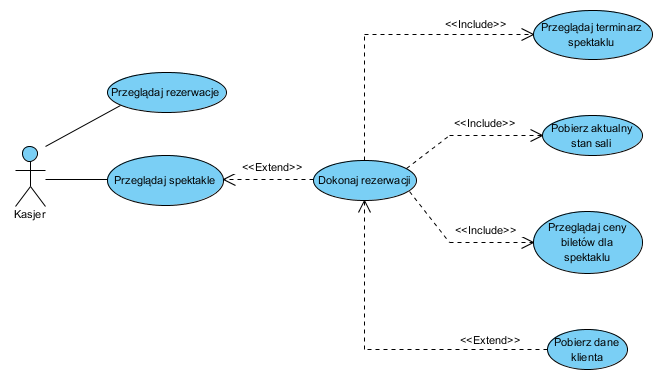
\includegraphics[width=0.75\textwidth]{images/diagram_pu.png}
	\caption{Diagram przypadków użycia}
	\label{fig:diagram_pu}
\end{figure}

W naszym systemie przewidziana została tylko jedna rola, jaką jest kasjer. Powinien on mieć możliwość przeglądania dokonanych rejestracji, a także wprowadzenia do systemu nowych. Przy opcji nowej rezerwacji, pracownik na podstawie informacji przekazanych przez klienta teatru, będzie miał możliwość wyboru sceny, terminu i wolnych miejsc na sali. Dokończenie procesu rezerwacji będzie wymagało wprowadzenia danych klienta. Jeżeli gość istnieje już w bazie danych, jego dane będzie można pobrać na podstawie adresu e-mail.

\section{Wymagania niefunkcjonalne}
Tworzona aplikacja ma być aplikacją webową. Umożliwi to użytkownikom dostęp do niej z niemal dowolnego urządzenia elektronicznego. Powinna być również responsywna, aby mimo różnych rozdzielczości ekranów zapewnić zadowalającą czytelność i funkcjonalność. Sam jej wygląd powinien być możliwie jak najprostszy, aby użytkownik nie czuł uczucia dyskomfortu podczas poruszania się po niej oraz by nie musiał poświęcić dużo czasu na nauczenie się jej obsługi.

\subsection{Wykorzystane technologie i narzędzia}
Dostęp  do  baz  danych  będzie  możliwy  za  pośrednictwem  odpowiednich  serwerów zarządzających bazami danych MySQL, a proces replikacji między nimi zostanie zrealizowany z wykorzystaniem programu MySQL Workbench. Ze stworzonego systemu baz danych będzie korzystać aplikacja webowa. Logika aplikacji była tworzona w języku Ruby. Natomiast warstwa prezentacji budowana była w HTML5, CSS3, Bootstrap, JavaScript i AngularJS. Do  specyfikacji  funkcji systemu wykorzystany zostanie język modelowania UML.

\subsection{Wymagania dotyczące rozmiaru bazy danych}
Baza danych stworzona zostanie do obsługi procesu rezerwacji biletów do teatru. Będzie to wymagało m.in. przechowywania danych o klientach, a także aktualnych rezerwacjach. Na stałe w bazie danych wprowadzone zostaną informacje o dostępnych salach. Informacje o aktualnie granych spektaklach, biletów na nie oraz terminarzu, nie będą wymagały dużej ilości miejsca. Najbardziej obciążone tabele bazy będą przechowywały dane klientów i rezerwacji. Zakładając, że w teatrze w danym okresie będzie granych kilka sztuk na różnych salach i w różnych terminach możemy spodziewać się, że dane o tym będą zapisane na co najmniej kilkaset rekordach. Jednakże informacje te będzie można usunąć po odbyciu się spektaklu, a więc baza danych nigdy nie powinna osiągnąć dużych rozmiarów.

\subsection{Wymagania dotyczące bezpieczeństwa systemu}
Najbardziej newralgiczne dane będą dotyczyły klientów teatru. W bazie będą przechowywane takie informacje jak numer telefonu, czy adres e-mail. Jednakże system został przeznaczony tylko dla pracowników teatru, a wcześniej wymienione dane nie są aż tak niebezpieczne by były dodatkowo szyfrowane. Dlatego przyjmujemy, że stworzony system nie wymaga dodatkowych zabezpieczeń.

\section{Przyjęte założenia projektowe}
W projekcie będzie zrealizowany 3-warstwowy model komunikacji klient/serwer w postaci tzw. „cienkiego klienta” (Rys. \ref{fig:system-diagram}). Dostęp  do  aplikacji  realizującej  funkcje  biznesowe  będzie realizowany poprzez podanie adresu serwera WWW. W projekcie zostaną wykorzystywane niejednorodne, relacyjne bazy danych.  Dostęp  do  systemu baz  danych  zostanie zrealizowany  w  oparciu  o funkcje aplikacji. Komunikacja w systemie baz danych będzie przebiegała zgodnie z modelem master slave. Zapis będzie możliwy tylko na serwer z rolą mastera, natomiast odczyt będzie możliwy z wszystkich trzech serwerów bazodanowych. W celu zrównoważenia obciążenia wykorzystany zostanie Load Balancing.

\begin{figure}[!ht]
	\centering
	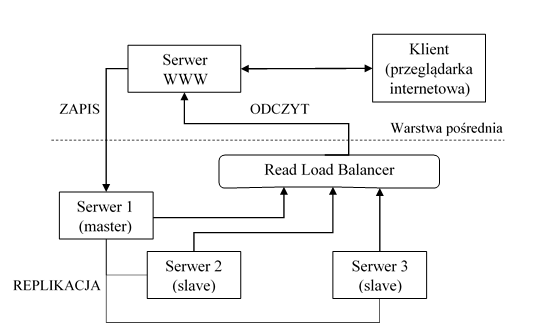
\includegraphics[width=0.7\textwidth]{images/struktura_systemu.png}
	\caption{Schemat systemu}
	\label{fig:system-diagram}
\end{figure}

\chapter{Podsumowanie pracy}
voluptas sit, aspernatur aut odit aut fugit, sed quia consequuntur magni dolores eos, qui ratione voluptatem sequi nesciunt, neque porro quisquam est, qui dolorem ipsum, quia dolor sit, amet, consectetur, adipisci velit, sed quia non numquam eius modi tempora incidunt, ut labore et dolore magnam aliquam quaerat voluptatem. Ut enim ad minima veniam, quis nostrum exercitationem ullam corporis suscipit laboriosam, nisi ut aliquid ex ea commodi consequatur? Quis autem vel eum iure reprehenderit, qui in ea voluptate velit esse, quam nihil molestiae consequatur, vel illum, qui dolorem eum fugiat, quo voluptas nulla pariatur?

Sed ut perspiciatis, unde omnis iste natus error sit voluptatem accusantium doloremque laudantium, totam rem aperiam eaque ipsa, quae ab illo inventore veritatis et quasi architecto beatae vitae dicta sunt, explicabo. Nemo enim ipsam voluptatem, quia voluptas sit, aspernatur aut odit aut fugit, sed quia consequuntur magni dolores eos, qui ratione voluptatem sequi nesciunt, neque porro quisquam est, qui dolorem ipsum, quia dolor sit, amet, consectetur, adipisci velit, sed quia non numquam eius modi tempora incidunt, ut labore et dolore magnam aliquam quaerat voluptatem. Ut enim ad minima veniam, quis nostrum exercitationem ullam corporis suscipit laboriosam, nisi ut aliquid ex ea commodi consequatur? Quis autem vel eum iure reprehenderit, qui in ea voluptate velit esse, quam nihil molestiae consequatur, vel illum, qui dolorem evoluptas sit, aspernatur aut odit aut fugit, sed quia consequuntur magni dolores eos, qui ratione voluptatem sequi nesciunt, neque porro quisquam est, qui dolorem ipsum, quia dolor sit, amet, consectetur, adipisci velit, sed quia non numquam eius modi tempora incidunt, ut labore et dolore magnam aliquam quaerat voluptatem. Ut enim ad minima veniam, quis nostrum exercitationem ullam corporis suscipit laboriosam, nisi ut aliquid ex ea commodi consequatur? Quis autem vel eum iure reprehenderit, qui in ea voluptate velit esse, quam nihil molestiae consequatur, vel illum, qui dolorem eum fugiat, quo voluptas nulla pariatur?

Sed ut perspiciatis, unde omnis iste natus error sit voluptatem accusantium doloremque laudantium, totam rem aperiam eaque ipsa, quae ab illo inventore veritatis et quasi architecto beatae vitae dicta sunt, explicabo. Nemo enim ipsam voluptatem, quia voluptas sit, aspernatur aut odit aut fugit, sed quia consequuntur magni dolores eos, qui ratione voluptatem sequi nesciunt, neque porro quisquam est, qui dolorem ipsum, quia dolor sit, amet, consectetur, adipisci velit, sed quia non numquam eius modi tempora incidunt, ut labore et dolore magnam aliquam quaerat voluptatem. Ut enim ad minima veniam, quis nostrum exercitationem ullam corporis suscipit laboriosam, nisi ut aliquid ex ea commodi consequatur? Quis autem vel eum iure reprehenderit, qui in ea voluptate velit esse, quam nihil molestiae consequatur, vel illum, qui dolorem evoluptas sit, aspernatur aut odit aut fugit, sed quia consequuntur magni dolores eos, qui ratione voluptatem sequi nesciunt, neque porro quisquam est, qui dolorem ipsum, quia dolor sit, amet, consectetur, adipisci velit, sed quia non numquam eius modi tempora incidunt, ut labore et dolore magnam aliquam quaerat voluptatem. Ut enim ad minima veniam, quis nostrum exercitationem ullam corporis suscipit laboriosam, nisi ut aliquid ex ea commodi consequatur? Quis autem vel eum iure reprehenderit, qui in ea voluptate velit esse, quam nihil molestiae consequatur, vel illum, qui dolorem eum fugiat, quo voluptas nulla pariatur?

Sed ut perspiciatis, unde omnis iste natus error sit voluptatem accusantium doloremque laudantium, totam rem aperiam eaque ipsa, quae ab illo inventore veritatis et quasi architecto beatae vitae dicta sunt, explicabo. Nemo enim ipsam voluptatem, quia voluptas sit, aspernatur aut odit aut fugit, sed quia consequuntur magni dolores eos, qui ratione voluptatem sequi nesciunt, neque porro quisquam est, qui dolorem ipsum, quia dolor sit, amet, consectetur, adipisci velit, sed quia non numquam eius modi tempora incidunt, ut labore et dolore magnam aliquam quaerat voluptatem. Ut enim ad minima veniam, quis nostrum exercitationem ullam corporis suscipit laboriosam, nisi ut aliquid ex ea commodi consequatur? Quis autem vel eum iure reprehenderit, qui in ea voluptate velit esse, quam nihil molestiae consequatur, vel illum, qui dolorem eję danych na stronie
internetowej, co zwiększa liczbę zastosowań systemu.
 
Dalszy rozwój projektu może zakładać:
\begin{itemize}
\item projekt obwodfgsgfsgudowy ursządzenigsdo-nadawczego,
\item optymalizagfdsgsgsfgso mają być
wyświetlane pomiary,
\item możliwsgfsdgfsów do pliku.
\item powiadamianie usgdfgsdfgczeniu mierzonej wielkości
fizycznej,
\item sterowaniesdgsdfgscję internetową.
\end{itemize}
 %utworzenie w
                                             %spisietresci pozycji
                                             %Bibliografia
  \begin{thebibliography}{9}
\addcontentsline{toc}{chapter}{Bibliografia}

  \bibitem{rfc2616} {\em Hypertext Transfer Protocol -- HTTP/1.1} 1999: 
  https://tools.ietf.org/html/rfc2616 (dostęp 09.12.2015 r.)

  \bibitem{ajax} {\em XMLHttpRequest Living Standard} 25.11.2015 r.: 
  https://xhr.spec.whatwg.org/ (dostęp 11.12.2015 r.)

  \end{thebibliography}
%\bibliography{bibliografia} % wstawia bibliografię korzystając z pliku
                            % bibliografia.bib - dotyczy BibTeXa,
                            % jeżeli nie korzystamy z BibTeXa należy
                            % użyć otoczenia thebibliography

%opcjonalnie może się tu pojawić spis rysunków i tabel
\listoffigures
\addcontentsline{toc}{chapter}{Spis rysunków}
 \listoftables
\addcontentsline{toc}{chapter}{Spis tabel}
% \listoflistings
 \lstlistoflistings
 \addcontentsline{toc}{chapter}{Spis listingów}

\end{document}
